\begin{figure*}
	\centering
	\small
	\begin{tabular}{ccc}
		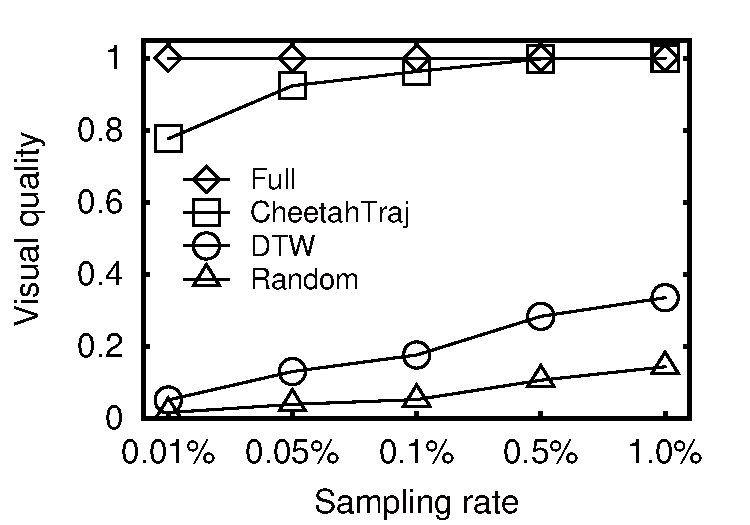
\includegraphics[width=0.22\linewidth]{pictures/quantitative_study/rate_porto_q}
		&
		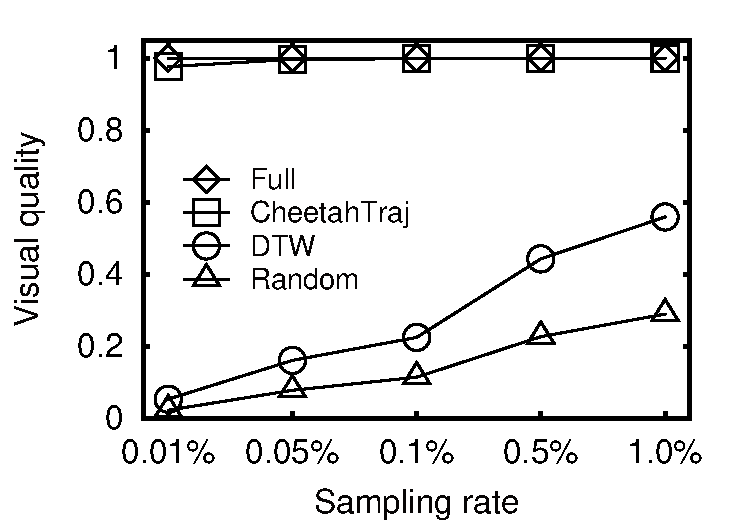
\includegraphics[width=0.22\linewidth]{pictures/quantitative_study/rate_sz_q}
        &
		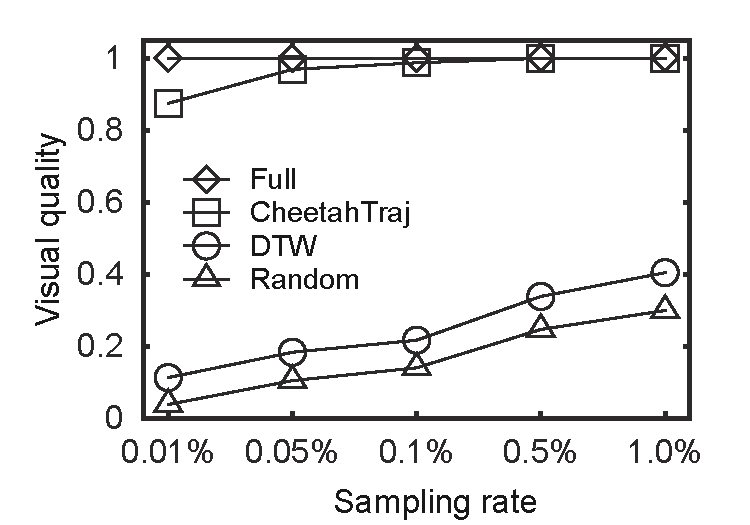
\includegraphics[width=0.22\linewidth]{pictures/quantitative_study/rate_cd_q}
		\\
		(A) \pt{}
		&
		(B) \sz{}
		&
		(C) \cd{}
	\end{tabular}
    \trim
    \vspace{-2mm}
	\caption{Effect of varying sampling rate visual quality.}
	\label{fig:rate_quality}
	\trim \trim
\end{figure*}

\if 0
\begin{figure*}
	\centering
	\small
	\begin{tabular}{ccc} 
		%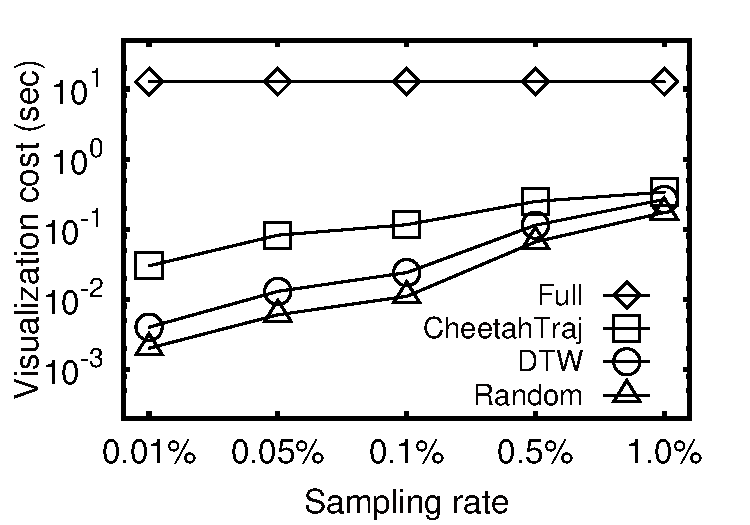
\includegraphics[width=0.22\linewidth]{pictures/quantitative_study/rate_porto_t}
		\includegraphics[width=0.22\linewidth]{pictures/quantitative_study/quality_time/tporto_log}
		&
		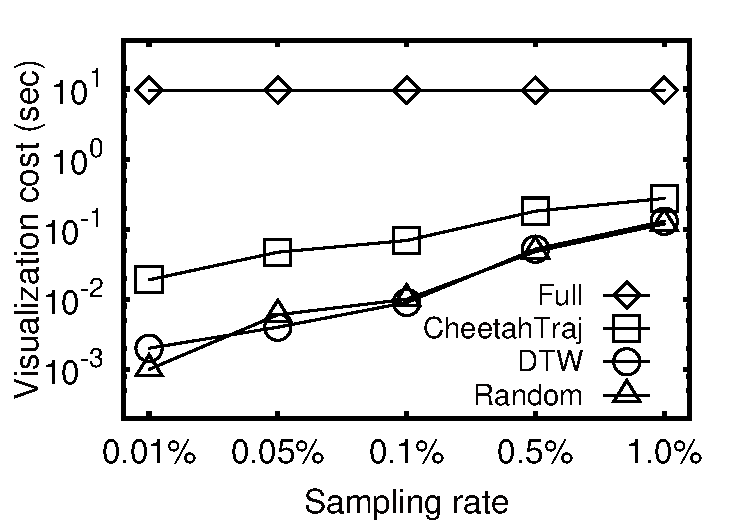
\includegraphics[width=0.22\linewidth]{pictures/quantitative_study/rate_sz_t}
        &
		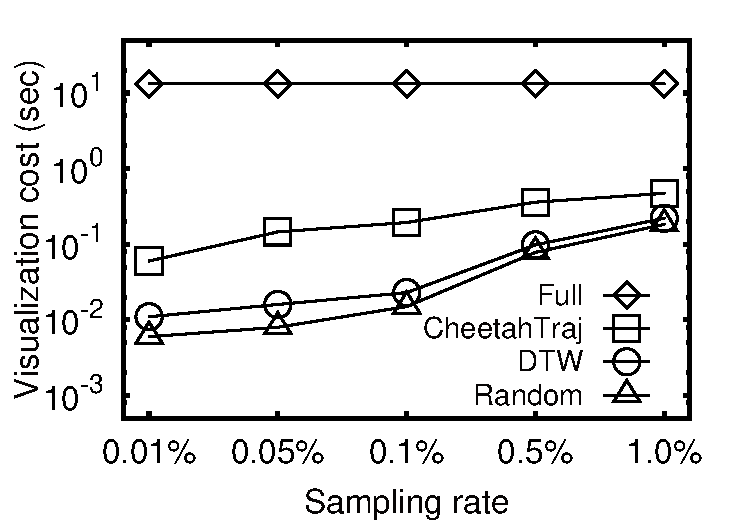
\includegraphics[width=0.22\linewidth]{pictures/quantitative_study/rate_cd_t}
		\\
		(A) \pt{}
		&
		(B) \sz{}
		&
		(C) \cd{}
	\end{tabular}
    \trim
    \vspace{-2mm}
	\caption{Effect of  sampling rate on visualization cost.}
	\label{fig:rate_vistime}
	\trim \trim
\end{figure*}
\fi
\begin{figure*}
	\centering
	\small
	\begin{tabular}{ccc} 
		\includegraphics[width=0.22\linewidth]{pictures/quantitative_study/quality_time/tporto}
		&
		\includegraphics[width=0.22\linewidth]{pictures/quantitative_study/quality_time/tshenzhen}
		&
		\includegraphics[width=0.22\linewidth]{pictures/quantitative_study/quality_time/tcd}
		\\
		(A) \pt{}
		&
		(B) \sz{}
		&
		(C) \cd{}
	\end{tabular}
	\trim
	\vspace{-2mm}
	\caption{Effect of  sampling rate on visualization cost.}
	\label{fig:rate_vistime}
	\trim \trim
\end{figure*}
\if 0
\begin{figure*}
	\centering
	\small
	\begin{tabular}{ccc}
		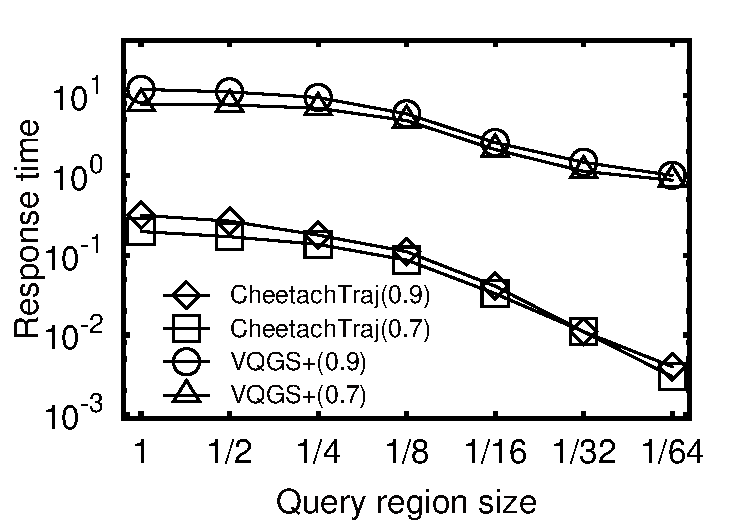
\includegraphics[width=0.22\linewidth]{pictures/quantitative_study/size_porto_t}
		&
		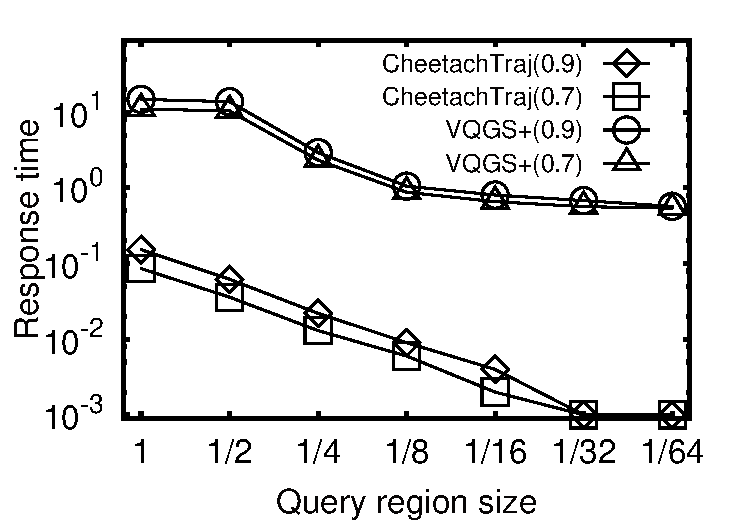
\includegraphics[width=0.22\linewidth]{pictures/quantitative_study/size_sz_t}
		&
		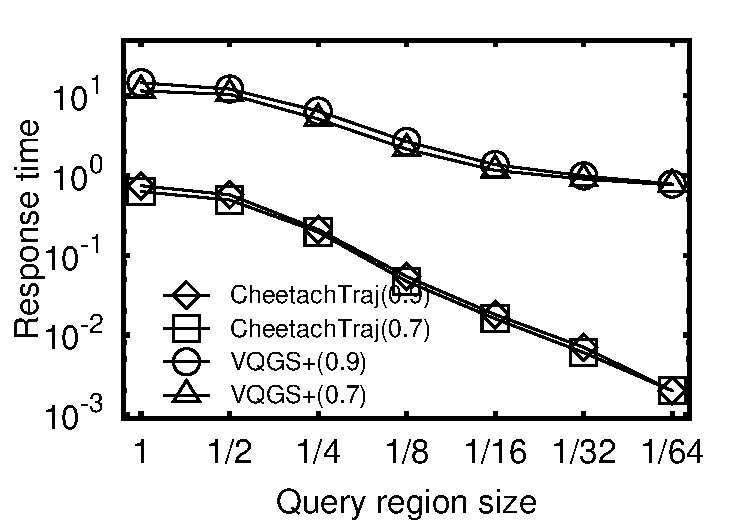
\includegraphics[width=0.22\linewidth]{pictures/quantitative_study/size_cd_t}
		\\
		(A) \pt{}
		&
		(B) \sz{}
		&
		(C) \cd{}
	\end{tabular}
    \trim
    \vspace{-2mm}
	\caption{Effect of region size on end-top-end response time.}
	\label{fig:size_responsetime}
	\trim \trim
\end{figure*}
\fi

\begin{figure*}
	\centering
	\small
	\begin{tabular}{ccc}
		\includegraphics[width=0.22\linewidth]{pictures/quantitative_study/regionsize_response_time/tporto}
		&
		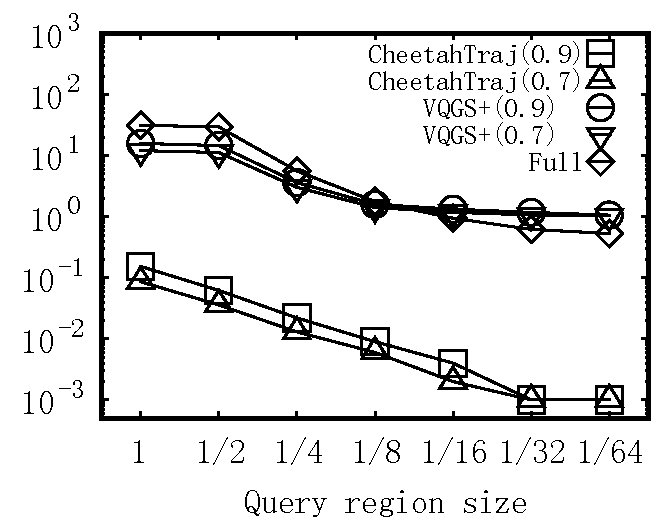
\includegraphics[width=0.22\linewidth]{pictures/quantitative_study/regionsize_response_time/tshenzhen}
		&
		\includegraphics[width=0.22\linewidth]{pictures/quantitative_study/regionsize_response_time/tcd}
		\\
		(A) \pt{}
		&
		(B) \sz{}
		&
		(C) \cd{}
	\end{tabular}
	\trim
	\vspace{-2mm}
	\caption{Effect of region size on end-top-end response time.}
	\label{fig:size_responsetime}
	\trim \trim
\end{figure*}

\begin{figure*}
	\centering
	\small
	\begin{tabular}{ccc}
		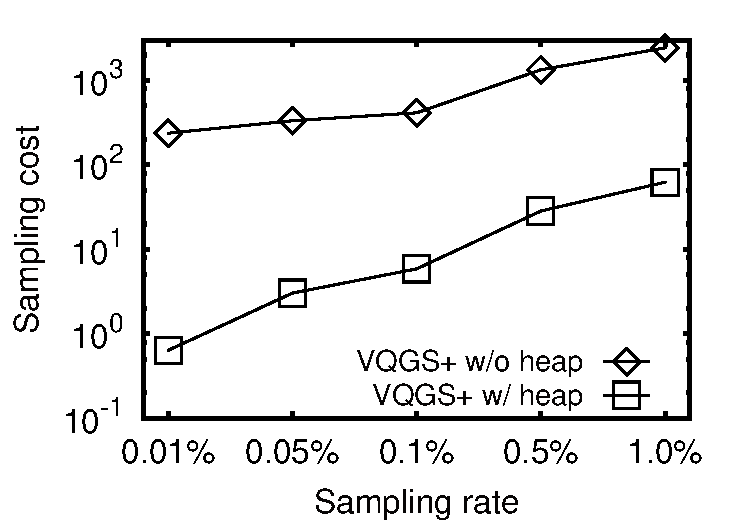
\includegraphics[width=0.22\linewidth]{pictures/quantitative_study/vqgs_porto_t}
		&
		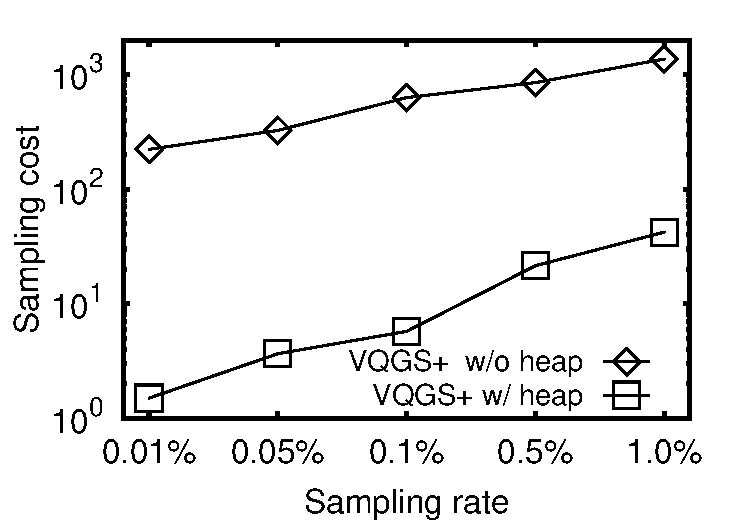
\includegraphics[width=0.22\linewidth]{pictures/quantitative_study/vqgs_sz_t}
		&
		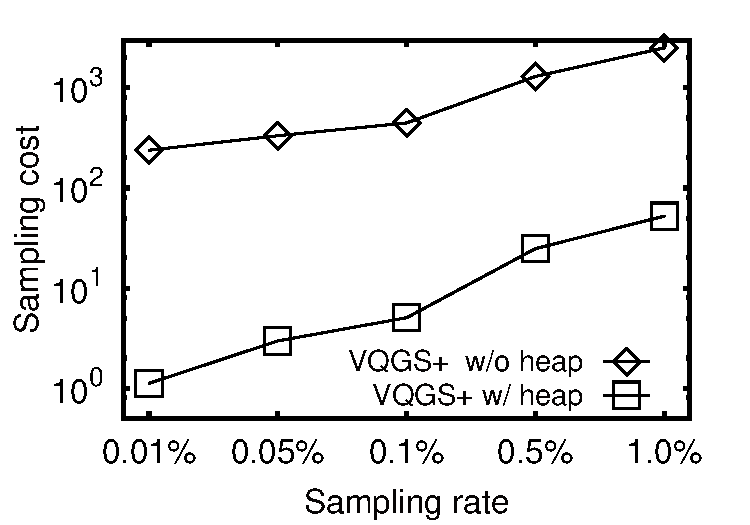
\includegraphics[width=0.22\linewidth]{pictures/quantitative_study/vqgs_cd_t}
		\\
		(A) \pt{}
		&
		(B) \sz{}
		&
		(C) \cd{}
	\end{tabular}
    \trim
	\caption{Effect of sampling rate on the sampling cost of $\vatss$ with/without optimization}
	\label{fig:rate_algtime}
	\trim \trim
\end{figure*}

\subsection{Quantitative Evaluation}\label{sec:quality}
In this part, we quantitatively evaluate the visual quality and efficiency of $\avats$ on the three real-world trajectory datasets.

\stitle{Visual quality} Figure~\ref{fig:rate_quality} reports the visualization quality (as defined in Equation~\eqref{eqref:loss}) of the methods under different sampling rate.
We consider the entire region in each dataset for this experiment.
The results show that our proposal $\avats$ achieves significantly higher quality than $\rand$ and $\mathsf{DTW}$ under the same sampling rate.
This is because the sampling algorithm $\vats$ and $\vatss$ in the $\avats$ framework are designed with explicit considerations for visual quality.
Specifically, the quality of $\avats$ approaches 1 when the sampling rate is still less than 1\% for all 3 datasets.
$\mathsf{DTW}$ has a higher quality than $\rand$ because it considers the diversity of trajectories.


In Figure~\ref{fig:rate_vistime}, we report the visualization cost (i.e., the wall clock time to generate visualization result using the sampled trajectories) for the methods under different sampling rate.
We still consider the entire region in this experiment and the visualization time of $\full$ (which does not change with sampling rate) is included at the top of each figure for reference.
The results show that all sampling methods achieve significantly shorter visualization cost than $\full$, and the speedup can be 1 to 4 orders of magnitude.
This confirms our observation that sampling is effective in improving visualization efficiency.
Under the same sampling rate, our $\avats$ takes slightly longer visualization time than $\rand$ and $\mathsf{DTW}$
because $\avats$ tends to select long trajectories for quality maximization.
%It is worth to point out the largest visualization cost of $\avats$ in \pt{}, \sz{} and \cd{} are 0.339, 0.275 and 0.471
Combining Figure~\ref{fig:rate_quality} and~\ref{fig:rate_vistime}, we can conclude that $\avats$ can achieve high visualization quality with  short visualization latency.


\stitle{Efficiency of $\avats$}
We evaluate the \textit{response time} of our $\avats$ framework under different quality guarantees and region sizes in Figure~\ref{fig:size_responsetime}.
The response time of $\avats$ is the end-to-end time for generating visualization for a selected region, which includes querying the $\avats$ index and computing the visualization.
For comparison, we also plot the response time of $\vatss$ (with $\delta\!=\!8$), which uses on-line sampling instead of querying the index in $\avats$ framework.
We constrain the regions to be rectangles with a constant height/width ratio and measure the size of a region by dividing its height over the height of the entire region.
For each region size, we report the average response time of three typical regions, i.e., a dense region, a sparse region and a medium region.
The results show that $\avats$ achieves a short response time (less than 1 second in all cases and 0.2 second for most cases) for different region sizes and quality guarantees. $\vatss$ is 1 to 2 orders of magnitude slower than $\avats$ and takes at most 14.802 seconds in all cases. These results show that $\vatss$ cannot support interactive visual exploration and the $\invQ$-tree index in $\avats$ is effective in improving efficiency.
In addition, the response time decreases rapidly when the region size shrinks as there are fewer trajectories in a smaller region.
However, the response time required to achieve a high quality (e.g., 0.9) is not significantly longer than a low quality (e.g., 0.7) as quality improves quickly with the number of sampled trajectories as a shown in Figure~\ref{fig:rate_quality}.





\stitle{Effect of heap-based lazy computation}
In Figure~\ref{fig:rate_algtime}, we report the running time of $\vatss$  with and without the heap-based lazy computation.
The results show that the heap-based optimization reduces the running time of $\vatss$ around 2 orders of magnitude.
For the sampling rates we considered, $\vatss$ runs efficiently and can finish within 1 second for the entire dataset.



%\begin{figure}[t]
%	\centering
%	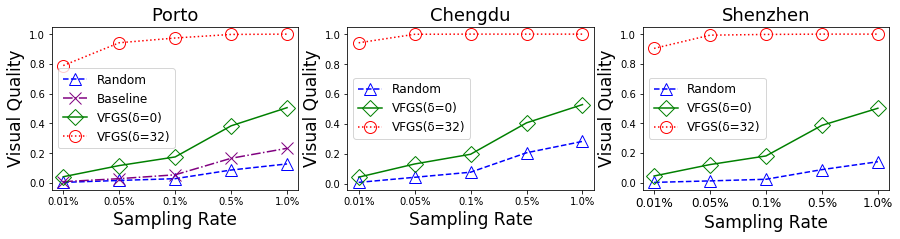
\includegraphics[width=0.5\textwidth]{pictures/quantitative_study_icde/sample_quality.png}
%	\vspace{-8mm}
%	\caption{Visual quality vs. sampling rates.}
%	\label{fig:sample_quality}
%	\vspace{-3mm}
%\end{figure}

%\begin{figure}[t]
%	\centering
%	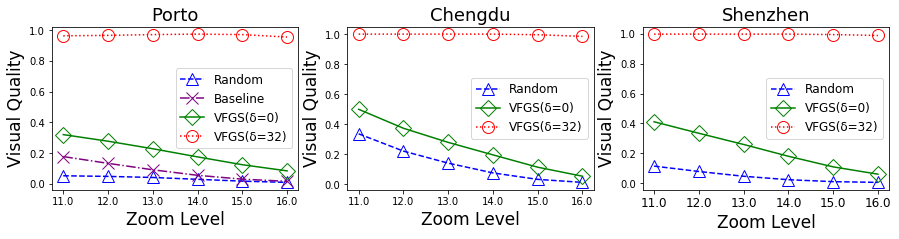
\includegraphics[width=0.5\textwidth]{pictures/quantitative_study_icde/zoom_quality.png}
%	\vspace{-8mm}
%	\caption{Visual quality vs. zoom level.}
%	\label{fig:zoom_quality}
%	\vspace{-3mm}
%\end{figure}


%\begin{table}
%	\centering
%	\small
%	\caption{The cost of $\invQ$-tree index}
%	\begin{tabular}{|@{}c@{}|@{}c@{}|@{}c@{}|@{}c@{}|@{}c@{}|} \hline
%		Dataset (size) & Height & Building time & Memory size \\ \hline
%		\pt{} (1.44G)	& 13 & 526.390s & 3.65GB  \\ \hline
%		\sz{} (1.02G)	& 13 & 435.291s  & 3.12GB \\ \hline
%		\cd{} (1.49G)	& 13 & 454.151s & 3.71GB \\ \hline
%	\end{tabular}	\label{tab:index cost}
%    \trim %\trim
%\end{table}

\begin{table}
	\centering
	\small
	\caption{The cost of $\invQ$-tree index}
	\vspace{-3mm}
	\begin{tabular}{|c|c|c|c|} \hline
		Dataset (size) & Height & Building time & Memory size \\ \hline
		\pt{} (1.44G)	& 13 & 526.390s & 3.65GB  \\ \hline
		\sz{} (1.02G)	& 13 & 435.291s  & 3.12GB \\ \hline
		\cd{} (1.49G)	& 13 & 454.151s & 3.71GB \\ \hline
	\end{tabular}	\label{tab:index cost}
	\trim %\trim
\end{table}

\stitle{$\invQ$-tree index cost evaluation}
We report the building time and memory cost of the $\invQ$-tree index in Table~\ref{tab:index cost}.
For all three datasets, it takes less than 10 minutes to build the $\invQ$ index with a height of 13.
The memory cost of the $\invQ$ index in the last column is also comparable with the size of the raw data shown in the first column.




%\stitle{Running time evaluation}

%\begin{figure}[t]
%	\centering
%	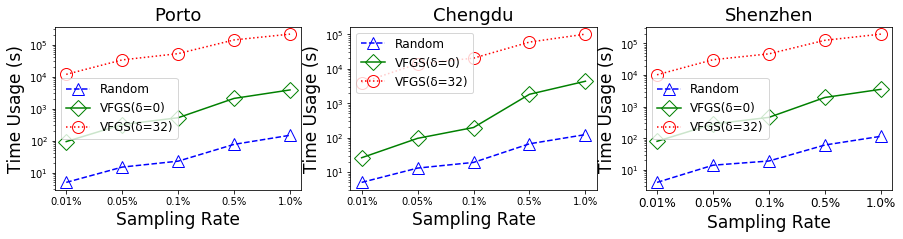
\includegraphics[width=0.5\textwidth]{pictures/quantitative_study_icde/sample_time.png}
%	\vspace{-8mm}
%	\caption{Time usage vs. sampling rates.}
%	\label{fig:sample_time}
%	\vspace{-3mm}
%\end{figure}

%\begin{figure}
%	\centering
%	\small
%	\begin{tabular}{cc}
%		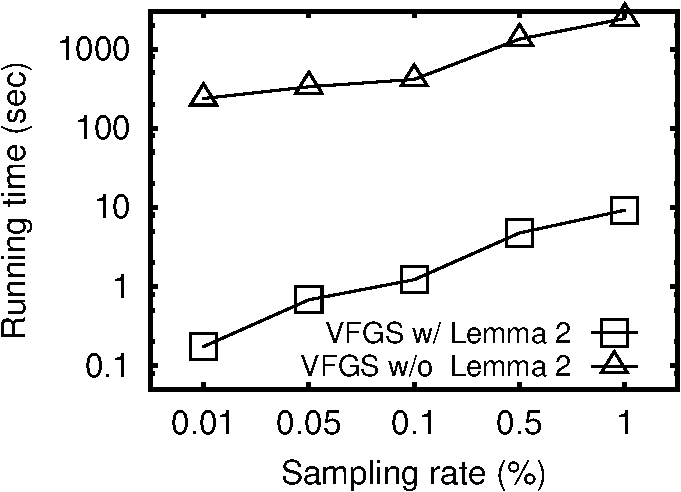
\includegraphics[width=0.44\columnwidth]{pictures/tporto}
%		&
%		\includegraphics[width=0.44\columnwidth]{pictures/tshenzhen}
%		\\
%		(A) \pt{}
%		&
%		(B) \sz{}	
%	\end{tabular}
%	\vspace{-3mm}
%	\caption{Running time of $\vats$ w/ and w/o Lemma~\ref{lem:submodular}.}
%	\label{fig:cost}
%	\vspace{-6mm}
%\end{figure}
%\QM{unfininshed}
%We first conduct an experiment to evaluate the rendering cost by datasize. We vary the number of trajectories from 1000 to 1 million, which are randomly selected from \pt{} dataset. The experimental results are summarized in Table~\ref{tab:gpu}. We observe that the rendering cost is linear with the input data trajectories.
%
%We first report the running time of our $\vats$ algorithm in Figure~\ref{fig:cost} by varying the sampling rate from $0.01\%$ to $1\%$. The results show that $\vats$ is quite slow without the submodularity of contribution value, which agrees with Lemma~\ref{lem:submodular} in Section~\ref{sec:opt}.
%Then we shown the total time usage with sampling rate as Figure~\ref{fig:sample_time}. {*******}
%
%The optimized $\vats$ (e.g., $\vats$ with Lemma~\ref{lem:submodular}) outperforms $\vats$ by one to three orders of magnitudes on both datasets. The result show that running time of our $\vats$ algorithm is below 1 second in most cases. We have shown that $\vats$ provides good visualization performance with a low sampling rate (e.g., $0.1\%$ or $1\%$) in Section 6.1 and 6.2,  and Table~\ref{tab:gpu} suggests that the rendering latency scales almost linearly with dataset cardinality. By significantly reducing the dataset cardinality with sampling, $\vats$ can effectively reduces the rendering latency to make interactive visualization possible without sacrificing visual quality. For example, rendering the full $\pt{}$ dataset takes about \QM{34 seconds}, with a sampling rate of $1\%$, $\vats$ can bring down the rendering latency to less than 1 second.


